\begin{solution}
 \begin{enumerate}
 
\item To estimate the truncation error (TE) for the Crank-Nicolson method, we first recall Taylor's theorem with
remainder, which states that a function $u(x)$ can be expanded in a series about the point
$c$:
\[
u(x) = u(c)+u_x(c)(x-c)+ \frac{u_{xx}(c)}{2!} (x-c)^2+ \frac{u_{xxx}(c)}{3!} (x-c)^3+� � �+\frac{u^{(n+1)}(c)(\xi)}{n!}(x-c)^{n+1}
\]

where $\xi$ is between $x$ and $c$. The last term is referred to as the remainder term or truncation error.

We write the equation at the point $(x_i, t_{j+\frac{1}{2}})$. To better understanding let see Crank-Nicolson Stencil.
\vspace{-0.65cm}
\begin{figure}[h]
	\centering
		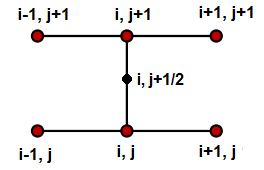
\includegraphics[width=.25\textwidth]{CN.png}
	\label{fig:CN}
	\caption{Crank-Nicolson Stencil}
\end{figure}

\newpage

Taylor series expansion of $u(x,t + \Delta t)$ around the point $(x, t+ \frac{\Delta t}{2})$ is
\begin{align*}
u(x,t + \Delta t) &= u(x, t+ \frac{\Delta t}{2}) + u_t(x, t+ \frac{\Delta t}{2}) \left(\frac{\Delta t}{2}\right)  + \frac{u_{tt}(x, t+ \frac{\Delta t}{2})}{2!}\left(\frac{\Delta t}{2}\right)^2 + \frac{u_{ttt}(x, t+ \frac{\Delta t}{2})}{3!}\left(\frac{\Delta t}{2}\right)^3\\ 
& + \frac{u_{tttt}(x, t+ \frac{\Delta t}{2})}{4!}\left(\frac{\Delta t}{2}\right)^4\ldots
\end{align*}
Similarly Taylor series expansion of $u(x,t)$ around the point $(x, t+ \frac{\Delta t}{2})$ is

\begin{align*}
u(x,t) &= u(x, t+ \frac{\Delta t}{2}) - u_t(x, t+ \frac{\Delta t}{2}) \left(\frac{\Delta t}{2}\right)  + \frac{u_{tt}(x, t+ \frac{\Delta t}{2})}{2!}\left(\frac{\Delta t}{2}\right)^2 - \frac{u_{ttt}(x, t+ \frac{\Delta t}{2})}{3!}\left(\frac{\Delta t}{2}\right)^3\\ 
& + \frac{u_{tttt}(x, t+ \frac{\Delta t}{2})}{4!}\left(\frac{\Delta t}{2}\right)^4\ldots 
\end{align*}

Taking difference of these two equations we get 

\begin{align*}
u(x,t + \Delta t)-u(x,t) &= 2 u_t(x, t+ \frac{\Delta t}{2}) \left(\frac{\Delta t}{2}\right) + 2 \frac{u_{ttt}(x, t+ \frac{\Delta t}{2})}{3!}\left(\frac{\Delta t}{2}\right)^3 \ldots 
\end{align*}
Dividing by $\Delta t$ both sides gives

\begin{equation}
\boxed{\frac{u(x,t + \Delta t)-u(x,t)}{\Delta t} =  u_t(x, t+ \frac{\Delta t}{2}) + \frac{1}{4} \frac{u_{ttt}(x, t+ \frac{\Delta t}{2})}{3!}\left(\Delta t\right)^2 \ldots}
\end{equation}

implying that the truncation error of the time derivative is $TE_{t}= \frac{1}{24}u_{ttt}(x, \eta)\left(\Delta t\right)^2$ such that $\eta \in(t, t+\Delta t)$. This implies the first order central finite difference formula for $\frac{\partial u}{\partial t}$ is $2$nd order accurate i.e., $O(\Delta t^2)$ accurate.



To approximate the term $u_{xx}(x, t+ \frac{\Delta t}{2} )$ we use the average of the second centered differences for $u_{xx}(x ,t+\Delta t)$ and $u_{xx}(x,t)$;

First of all let's find $u_{xx}(x ,t+\Delta t)$. Then Taylor series expansion of $u(x+\Delta x, t + \Delta t)$ around the point $(x, t+\Delta t)$ is (Note that we are expanding in $x$ direction at the $t+\Delta t$ th time level)

\begin{align*}
u(x + \Delta x,t + \Delta t) &= u(x, t+ \Delta t) + u_x(x, t + \Delta t) \left(\Delta x\right)  + \frac{u_{xx}(x, t + \Delta t)}{2!}\left(\Delta x\right)^2 + \frac{u_{xxx}(x, t + \Delta t)}{3!}\left(\Delta x\right)^3\\ 
& + \frac{u_{xxxx}(x, t + \Delta t)}{4!}\left(\Delta x\right)^4 + \frac{u_{xxxxx}(x, t + \Delta x)}{5!}\left(\Delta x\right)^5 \ldots
\end{align*}
Similarly Taylor series expansion of $u(x-\Delta x,t+ \Delta t)$ around the point $(x, t+ \Delta t)$ is

\begin{align*}
u(x - \Delta x,t + \Delta t) &= u(x, t+ \Delta t) - u_x(x, t + \Delta t) \left(\Delta x\right)  + \frac{u_{xx}(x, t + \Delta t)}{2!}\left(\Delta x\right)^2 - \frac{u_{xxx}(x, t + \Delta t)}{3!}\left(\Delta x\right)^3\\ 
& + \frac{u_{xxxx}(x, t + \Delta t)}{4!}\left(\Delta x\right)^4 - \frac{u_{xxxxx}(x, t + \Delta x)}{5!}\left(\Delta x\right)^5 \ldots
\end{align*}

Adding last two equation gives 

\begin{align*}
u(x + \Delta x,t + \Delta t) + u(x - \Delta x,t + \Delta t) &= 2u(x, t+ \Delta t) + u_{xx}(x, t + \Delta t)\left(\Delta x\right)^2 + 2 \frac{u_{xxxx}(x, t + \Delta t)}{4!}\left(\Delta x\right)^4 \ldots
\end{align*}

Subtracting $2u(x, t+ \Delta t)$ from both sides and dividing by $\Delta x^2$ gives

\begin{align*}
\underbrace{\frac{u(x + \Delta x,t + \Delta t)- 2u(x, t+ \Delta t)+ u(x - \Delta x,t + \Delta t)}{\Delta x^2}}_{=U^{j+1}} &= u_{xx}(x, t + \Delta t) + \frac{u_{xxxx}(x, t + \Delta t)}{12}\left(\Delta x\right)^2 \ldots
\end{align*}

Now we will find Taylor series expansion of $u(x+\Delta x, t)$ and $u(x-\Delta x, t)$  around the point $(x, t)$ (Note that this time we are getting Taylor series expansion in $x$ direction at the $t$ th time level). By repeating same procedure as $t+\Delta t$ th time level we get

\begin{align*}
\underbrace{\frac{u(x + \Delta x,t)- 2u(x, t+ \Delta t)+ u(x - \Delta x,t)}{\Delta x^2}}_{=U^{j}} &= u_{xx}(x, t) + \frac{u_{xxxx}(x, t)}{12}\left(\Delta x\right)^2 \ldots
\end{align*}

Now taking average of the second centered differences for $u_{xx}(x ,t+\Delta t)$ and $u_{xx}(x,t)$ we will find approximation for $u_{xx}(x, t+ \frac{\Delta}{2})$

\begin{equation}
\boxed{\frac{1}{2}(U^{j+1} + U^{j})= u_{xx}(x, t+\frac{\Delta t}{2}) + \frac{u_{xxxx}(x, t+\frac{\Delta t}{2})}{12}\left(\Delta x\right)^2 \ldots}
\end{equation}

implying that the truncation error of the 2nd order space derivative is $TE_{xx}= \frac{1}{12}u_{xxxx}(\xi, \eta)\left(\Delta x \right)^2$ such that $\eta \in(t, t+\Delta t)$ and $\xi \in (x-\Delta x , x+ \Delta x)$. This implies the 2nd order central finite difference formula for $\frac{\partial^2 u}{\partial x^2}$ is $2$nd order accurate i.e., $O(\Delta x^2)$ accurate.



Both (1) and (2) implies(subtracting (2) from (1)) 
\begin{equation*}
\underbrace{u_t(x, t+ \frac{\Delta t}{2})-u_{xx}(x, t+\frac{\Delta t}{2})}_{PDE} + TE_t - TE_{xx}=  \underbrace{\frac{u(x,t + \Delta t)-u(x,t)}{\Delta t} -\frac{1}{2}(U^{j+1} + U^{j})}_{Crank Nicolson} 
\end{equation*}
From here we can conclude 
\[|PDE-\text{Crank Nicolson}|= O(\Delta x^2 + \Delta t^2)\]
\begin{center}
\textbf{\emph{The following is another possible method to show the order of approximation, following Jesse's hint on Piazza.}}
\end{center}

It is possible to simplify the above derivation by proceeding in two steps.  Let us define the finite difference approximation to the second derivative
\[
FD(x,t) = \frac{u(x-\Delta x,t) - 2u(x,t) + u(x+\Delta x,t)}{\Delta x^2}.
\]
Then, let us define the average of the \emph{exact} second derivative
\[
D_{\rm avg}(x,t+\Delta t/2) = \frac{1}{2}\left( \pd{u(x,t+\Delta t)}{x}{2} + \pd{u(x,t)}{x}{2}\right).
\]
Then, showing 
\[
\left| \pd{u(x,t+\Delta t/2}{x}{2} - \frac{1}{2}(FD(x,t+\Delta t) + FD(x,t))\right|
\]
can be recast as showing
\begin{align*}
\left| \pd{u(x,t+\Delta t/2}{x}{2} - D_{\rm avg}(x,t+\Delta t/2)
+ D_{\rm avg}(x,t+\Delta t) - \frac{1}{2}(FD(x,t+\Delta t) + FD(x,t))\right|.
\end{align*}
We can then analyze the terms
\[
\pd{u(x,t+\Delta t/2}{x}{2} - D_{\rm avg}(x,t+\Delta t/2)
\]
and
\[
D_{\rm avg}(x,t+\Delta t) - \frac{1}{2}(FD(x,t+\Delta t) + FD(x,t))
\]
separately.  Expanding out the latter gives
\[
\frac{1}{2}\left( \pd{u(x,t+\Delta t)}{x}{2} + \pd{u(x,t)}{x}{2}\right) - \frac{1}{2}(FD(x,t+\Delta t) + FD(x,t)).
\]
Since the finite difference approximation to the second derivative is $O(\Delta x^2)$ accurate at $t$ and $t+\Delta t$, we know
\begin{align*}
D_{\rm avg}(x,t+\Delta t)& - \frac{1}{2}(FD(x,t+\Delta t) + FD(x,t)) \\
&= \frac{1}{2}\left( \pd{u(x,t+\Delta t)}{x}{2} + \pd{u(x,t)}{x}{2}\right) - \frac{1}{2}(FD(x,t+\Delta t) + FD(x,t))\\
&= \frac{1}{2}\left( \pd{u(x,t+\Delta t)}{x}{2} -FD(x,t+\Delta t)\right) + \frac{1}{2}\left(\pd{u(x,t)}{x}{2}-FD(x,t))\right)\\
&= O(\Delta x^2) +  O(\Delta x^2) =  O(\Delta x^2).
\end{align*}
Then, all that remains to do is to show
\[
\pd{u(x,t+\Delta t/2)}{x}{2} - D_{\rm avg}(x,t+\Delta t/2) = O(\Delta t^2).
\]
We can do this by expanding $\pd{u(x,t+\Delta t)}{x}{2}$ and $\pd{u(x,t)}{x}{2}$ out in a Taylor series \emph{in time} around the point $t + \Delta t/2$.  Then, 
\[
\pd{u(x,t+\Delta t)}{x}{2} = \pd{u(x,t+\Delta t/2)}{x}{2} + \pd{}{t}{}\pd{u(x,t+\Delta t/2)}{x}{2} \frac{\Delta t}{2} + \pd{}{t}{2}\pd{u(x,t+\Delta t/2)}{x}{2} \left(\frac{\Delta t}{2} \right)^2 + \ldots
\]
and
\[
\pd{u(x,t)}{x}{2} = \pd{u(x,t+\Delta t/2)}{x}{2} - \pd{}{t}{}\pd{u(x,t+\Delta t/2)}{x}{2} \frac{\Delta t}{2} + \pd{}{t}{2}\pd{u(x,t+\Delta t/2)}{x}{2} \left(\frac{\Delta t}{2} \right)^2 + \ldots.
\]
Adding these two together cancels out the Taylor series' second term 
\[
\pd{}{t}{}\pd{u(x,t+\Delta t/2)}{x}{2} \frac{\Delta t}{2},
\]
and dividing their sum by 2 gives 
\[
\frac{1}{2}\left(\pd{u(x,t+\Delta t)}{x}{2} + \pd{u(x,t)}{x}{2}\right) = \pd{u(x,t+\Delta t/2)}{x}{2} + \pd{}{t}{2}\pd{u(x,t+\Delta t/2)}{x}{2} \left(\frac{\Delta t}{2} \right)^2 + \ldots
\]
implying that $\pd{u(x,t+\Delta t/2)}{x}{2} - D_{\rm avg}(x,t+\Delta t/2) = O(\Delta t^2)$.  

\item From the problem Crank-Nicolson scheme given by following formula
\[
\frac{u_i^{j+ 1}-u_i^{j}}{dt} = \frac{1}{2}\left[\frac{u_{i+1}^{j+1} - 2u_i^{j+1} + u_{i-1}^{j+1}}{h^2} + \frac{u_{i+1}^{j} - 2u_i^{j} + u_{i-1}^{j}}{h^2}\right]
\] 
Define $$r= \frac{dt}{2 dx^2}.$$
Then it turns out
\[
u_i^{j+ 1}-u_i^{j} = r \left[u_{i+1}^{j+1} - 2u_i^{j+1} + u_{i-1}^{j+1} +  u_{i+1}^{j} - 2u_i^{j} + u_{i-1}^{j}\right]
\]

Rearranging the term gives

\[
(1+2r)u_i^{j+ 1}-r (u_{i+1}^{j+1}+ u_{i-1}^{j+1})   =  (1-2r) u_i^{j} + r (u_{i+1}^{j} + u_{i-1}^{j})
\]

This leads to following  matrix equation (since we had homogeneous Dirichlet boundary conditions we do not have any contribution to our system from Dirichlet boundary)

\begin{align*}
 \underbrace{\left[\begin{array}{rrrrr}
              1+2r & -r \\[0.25em]
               -r &  1+2r & -r \\
                 &  -r  &  1+2r & \ddots \\
                 & & \ddots & \ddots & -r \\[0.25em]
                 & & & -r &  1+2r 
               \end{array}\right]}_{\bf{L}}
          \underbrace{\left[\begin{array}{c} u_1^{j+ 1} \\[0.25em] u_2^{j+ 1} \\[0.25em] \vdots \\[0.25em] u_{N-1}^{j+ 1} \\[0.25em] u_N^{j+ 1} \end{array}\right]}_{U^{j+1}}
 = \\
  \underbrace{\left[\begin{array}{rrrrr}
              1-2r & r \\[0.25em]
               r &  1-2r & r \\
                 &  r  &  1-2r & \ddots \\
                 & & \ddots & \ddots & r \\[0.25em]
                 & & & r &  1-2r 
               \end{array}\right]}_{\bf{M}}
           \underbrace{\left[\begin{array}{c} u_1^{j} \\[0.25em] u_2^{j} \\[0.25em] \vdots \\[0.25em] u_{N-1}^{j} \\[0.25em] u_N^{j} \end{array}\right]}_{U^j}
\end{align*}
Then we have system of equations  $\bf{L} U^{j+1}=\bf{M} U^{j} $ or $ U^{j+1}= \bf{L}^{-1}\bf{M} U^{j} $ . Now we want to write $\bf{L}$ as sum of identity matrix $I$.
$$\bf{L}= I + \bf{A}$$ where $\bf{A}$ is

\[
r \left[\begin{array}{rrrrr}
              2 & -1 \\[0.25em]
               -1 &  2 & -1 \\
                 &  -1  &  2 & \ddots \\
                 & & \ddots & \ddots & -1 \\[0.25em]
                 & & & -1 &  2 
               \end{array}\right]
\]

Similarly we want to write $\bf{M}$ as sum of identity matrix $I$. $$\bf{M}= I - \bf{B}$$ where $\bf{B}$ is

\[
r \left[\begin{array}{rrrrr}
              2 & -1 \\[0.25em]
               -1 &  2 & -1 \\
                 &  -1  &  2 & \ddots \\
                 & & \ddots & \ddots & -1 \\[0.25em]
                 & & & -1 &  2 
               \end{array}\right]
\]

We can conclude $\bf{A}=\bf{B}$.

\item For the motivation first remember for any  timestepping method, \[
{\bf u}^{j+1} = (({{\bf I} + {\bf A}})^{-1} ({{\bf I} - {\bf B}}))^{j+1} {\bf u}^{0}
\]
where $u^0$ is initial value and it contain some error with our assumption. Define error $e^0 = |u^0-u_{*}^0|$  where $u_{*}$ is exact solution of the problem. Then $$e^j = |u^j-u_{*}^j|= |(({{\bf I} + {\bf A}})^{-1} ({{\bf I} - {\bf B}}))^{j} {\bf e}^{0}|.$$ Now taking norm of both sides

\begin{align*}
\|e^j\| &=\| (({{\bf I} + {\bf A}})^{-1} ({{\bf I} - {\bf B}}))^{j} {\bf e}^{0}\|\\
\mbox{(by matrix and vector norm property)} & \leq \| (({{\bf I} + {\bf A}})^{-1})^{j}\| \| ({{\bf I} - {\bf B}})^{j}\| \| {\bf e}^{0}\|\\
\mbox{(we know that} \|A^j\|\leq \|A\|^j) &\leq \|({{\bf I} + {\bf A}})^{-1}\|^j \|{{\bf I} - {\bf B}})\|^j \| {\bf e}^{0}\|
\end{align*}

We might define matrix norm as follows
\[
\| \bf A \| = \sqrt{\rho (\bf A \bf A^T)}=\sqrt{max |\lambda_i|^2} = max |\lambda_i|
\] where $\rho({\bf A})$ is called spectral radius of $\bf A$ which means maximum eigenvalues $\lambda$ of the matrix $ \bf A$.

Then we can say
\[ \|e^j\|\leq \left(|\lambda_{({\bf I+\bf A})^{-1}}| |\lambda_{({\bf I} - {\bf B})}|\right)^j \| {\bf e}^{0}\|
\]
If max eigenvalue of $({\bf I+\bf A}^{-1})({\bf I-\bf B})$ in modulus is less than one, then $e^j \rightarrow 0$ for $j \rightarrow \infty$ 
Now, by formula eigenvalues of the $N\times N$ matrices $\bf A $ and $\bf B$ is $ r(2+2 \cos \frac{i \pi}{N+1})= 4r \cos^2 \frac{i \pi}{2(N+1)} $  

Then $$|\lambda_{({\bf I+\bf A})^{-1}}|= |(1+4r \cos^2 \frac{i \pi}{2(N+1)})^{-1}|=\frac{1}{|1+4r \cos^2 \frac{i \pi}{2(N+1)}|}$$ and  $$|\lambda_{({\bf I-\bf B})}|= |(1-4r \cos^2 \frac{i \pi}{2(N+1)})|$$

Therefore
\[
|\lambda_{({\bf I+\bf A})^{-1}}| |\lambda_{({\bf I} - {\bf B})}| =\frac{|(1-4r \cos^2 \frac{i \pi}{2(N+1)})|}{|1+4r \cos^2 \frac{i \pi}{2(N+1)}|} \leq 1
\]

It is easy to see that above ratio is always less than one without any restriction on $r>0$. Then we say that Crank-Nicolson is unconditionally stable. \emph{Note: Students does not have to explain motivation part}.  

\begin{center}
\textbf{\emph{The following is another possible method to show stability, more tailored to Jesse's class and lectures.}}
\end{center}
From class, we note that it suffices to show that, since 
\[
u^j = (I + \bf{A})^{-1}(I-\bf{B})u^{j-1} = (I + \bf{A})^{-1}(I-\bf{B})^j u^{0},
\]
in order for $u^j$ to not blow up, $(I + \bf{A})^{-1}(I-\bf{B})^j$ must have eigenvalues with magnitude $<1$.  We note that $\bf A = \bf B = \frac{dt}{2}A$, where
\[
A = {\kappa \over h^2}\left[\begin{array}{rrrrr}
              2 & -1 \\[0.25em]
               -1 &  2 & -1 \\
                 &  -1  &  2 & \ddots \\
                 & & \ddots & \ddots & -1 \\[0.25em]
                 & & & -1 &  2 
               \end{array}\right],
\]
Then, recall from Problem 1 that $A$ is positive definite, and thus has eigenvalues $\lambda_i > 0$, so that ${\bf A} = \frac{dt}{2}A$ has eigenvalues $\frac{dt}{2}\lambda_i > 0$. Since the actual eigenvalue is not important (only that it is positive) we will simply refer to the eigenvalues of ${\bf A} = {\bf B}$ as $\mu_i$. 

Since $I + {\bf A} = I + \frac{dt}{2}A$ and $I - {\bf B} = I - \frac{dt}{2}A$ both have the same eigenvectors, they have the following eigenvalue decompositions
\[
(I + {\bf A})^{-1} = V\Lambda^{-1} V^T, \qquad \Lambda^{-1}_{ii} = \frac{1}{1+\mu_i}
\]
and
\[
(I - {\bf B}) = V\tilde{\Lambda}^{-1} V^T, \qquad \tilde{\Lambda}^{-1}_{ii} = 1-\mu_i
\]
where $\Lambda^{-1}_{ii}$ and $\tilde{\Lambda}_{ii}$ refer to the $i$th diagonal entry of the eigenvalue matrices.  As a result, 
\[
(I + {\bf A})^{-1}(I - {\bf B}) = V\Lambda^{-1}V^T V \tilde{\Lambda}V^T = V\Lambda^{-1}\tilde{\Lambda}V^T.
\]
Since $\Lambda^{-1}\tilde{\Lambda}$ is again a diagonal matrix, $V\Lambda^{-1}\tilde{\Lambda}V^T$ is an eigenvalue decomposition of $(I + {\bf A})^{-1}(I - {\bf B})$, with eigenvalues
\[
\frac{1-\mu_i}{1+\mu_i}, \quad i = 1,\ldots n. 
\]
Since $\mu_i > 0$, the above quantity always satisfies $\left|\frac{1-\mu_i}{1+\mu_i} \right| < 1$, the eigenvalues of $(I + {\bf A})^{-1}(I - {\bf B})$ have magnitude $<1$ and will thus not blow up as $j\rightarrow \infty$.  

\vspace{1em}

\item From part b we know that by solving following linear system we get solution successive time steps.
\[ U^{j+1}= ({{\bf I} + {\bf A}})^{-1} ({{\bf I} - {\bf B}}) U^{j} \]

From the graph note that when we use bigger time step heat equation converge to steady state case.

Included is Matlab code that can be used to generate the finite difference solution and the error between it and the exact solution.   
 \lstinputlisting{CN.m}
\begin{figure}
\centering
\subfigure[{FD solutions for various time level when $N=8$}]{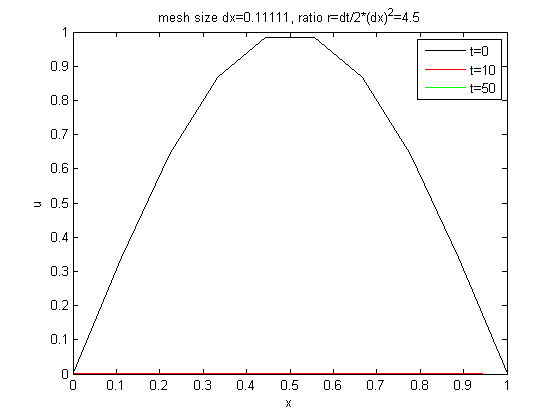
\includegraphics[width=.45\textwidth]{N_8.png}}
\subfigure[{FD solutions for various time level when $N=16$ }]{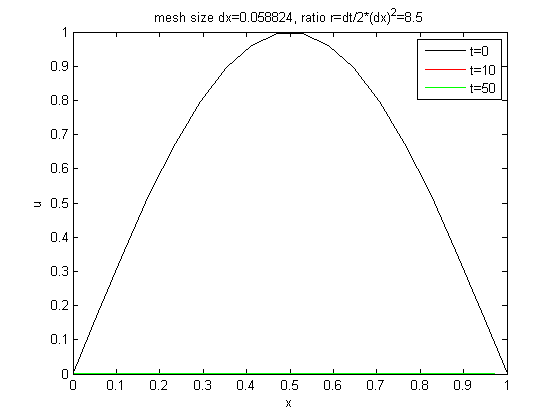
\includegraphics[width=.45\textwidth]{N_16.png}}
\end{figure} 


\begin{figure}
\centering
\subfigure[{FD solutions for various time level when $N=32$}]{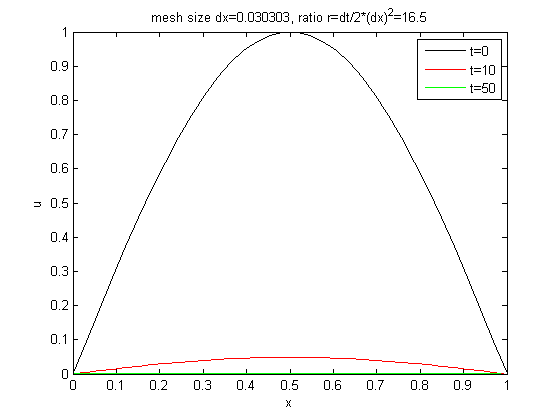
\includegraphics[width=.45\textwidth]{N_32.png}}
\subfigure[{FD surface plot when $N=8$ }]{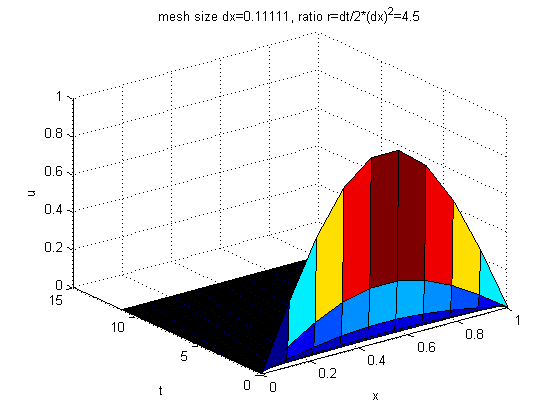
\includegraphics[width=.45\textwidth]{N_8surf.png}}
\end{figure} 

\begin{figure}
\centering
\subfigure[{FD surface plot when $N=16$}]{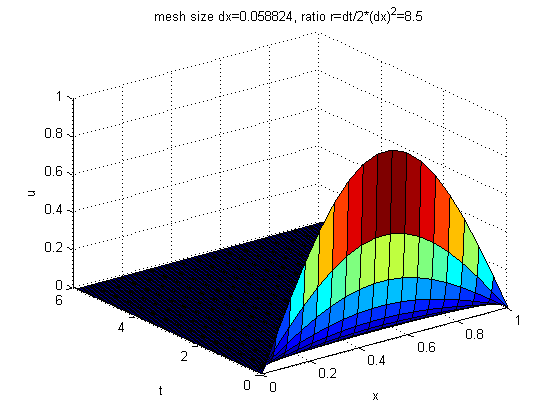
\includegraphics[width=.45\textwidth]{N_16surf.png}}
\subfigure[{FD surface plot when $N=32$ }]{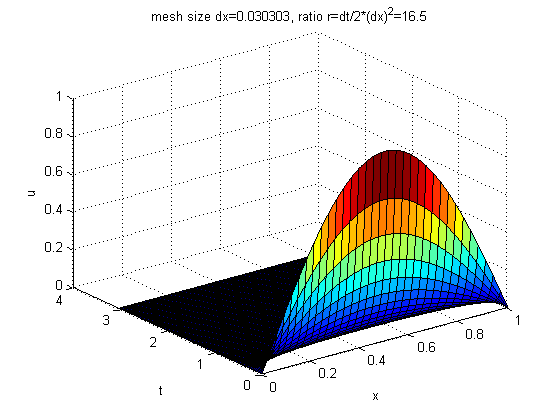
\includegraphics[width=.45\textwidth]{N_32surf.png}}
\end{figure} 


%\begin{figure}
%\centering
%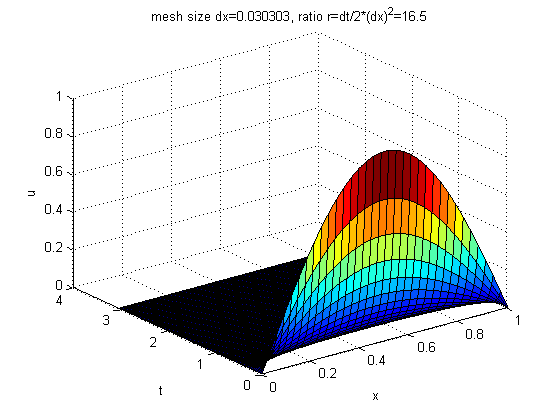
\includegraphics[width=.8\textwidth]{N_32surf.png}
%\caption{Finite difference solutions for various time level when $N=32$}
%\end{figure}

\emph{Note: Students does not have to give both FD 2D-plots and surfaces, one of them should be enough. Also the students who fix $dt$ and find solution is also excepted as a right solution. The plots with fix $dt$ is given end of that question.}

\item In that part note that $dt=h=\frac{1}{N+1}$ whenever we change $N$, $dt$ is also changing. For example when $N=32$ error is scaling with $10^{-4}$, $N=16$ error is scaling with $10^{-5}$ and $N=8$ error is scaling with $10^{-6}$ after $50$ time step. What's happening here, when $N=32$, $dt=1/33$, after $50$ time step we get total time $t=dt*100=1,5151$ similarly when $N=16$, $dt=1/17$ and after $50$ time step we get total time $t=dt*100=2,94$. This means that, actually we are calculating error later time step that's why, as we get bigger mesh size, error is getting better because we are finding error later time. It might be better comparison if we would fix $dt$ and looking at error when we proceed in time.

We added also the plot when $dt=0.001$ for the given method at that part. Here we can see we have better approximation when we increase $N$. 


\emph{Note: It is not expect from students to give above explanation and for the graph they do not have to plot loglog graph. Error plot would be enough. Also the students who fix $dt$ and find error is also excepted as a right solution.}

\begin{figure}
\centering
\subfigure[{FD error for various time level when $N=8$}]{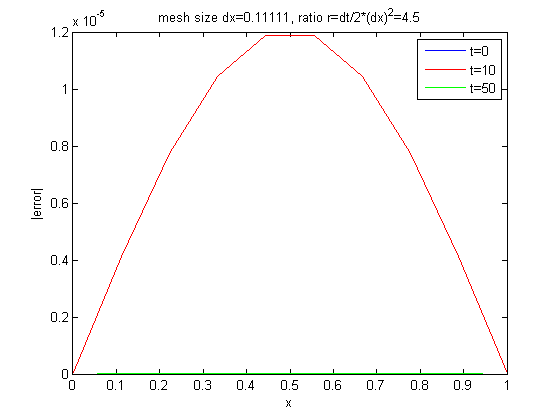
\includegraphics[width=.45\textwidth]{N_8error.png}}
\subfigure[{FD error for various time level when $N=16$ }]{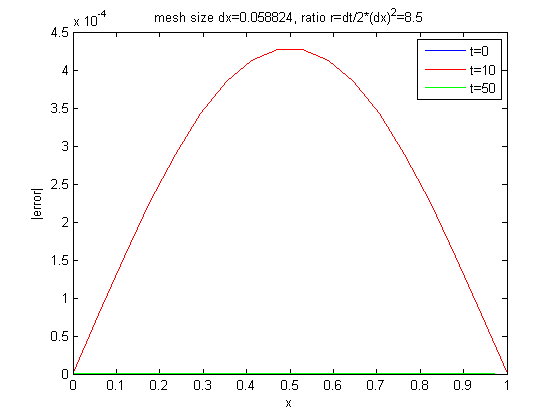
\includegraphics[width=.45\textwidth]{N_16error.png}}
\end{figure} 

\begin{figure}
\centering
\subfigure[{FD error for various time level when $N=32$}]{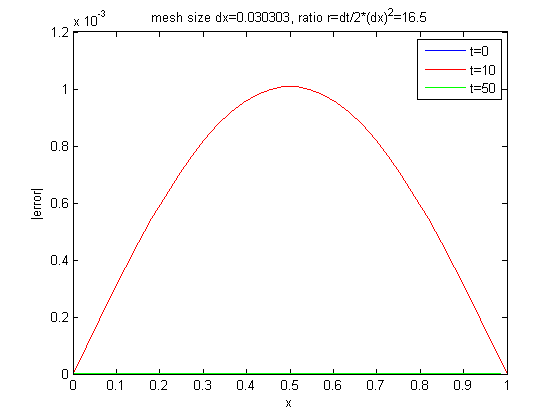
\includegraphics[width=.45\textwidth]{N_32error.png}}
\subfigure[{FD logerror for various time level when $N=8$ }]{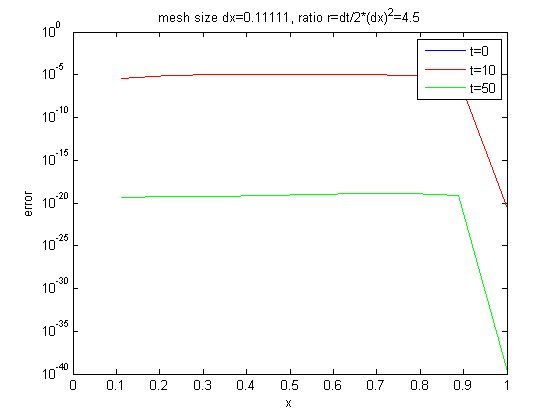
\includegraphics[width=.45\textwidth]{N_8logerror.png}}
\end{figure}

%\begin{figure}
%\centering
%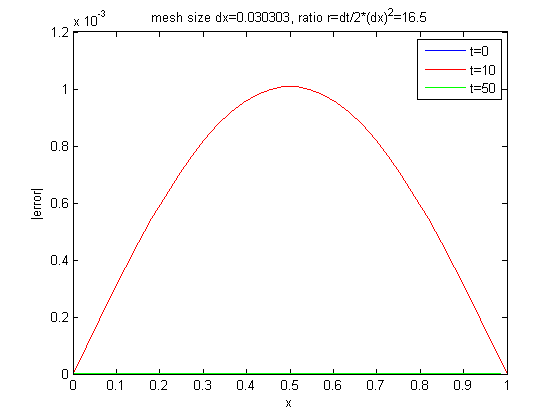
\includegraphics[width=.8\textwidth]{N_32error.png}
%\caption{FD error for various time level when $N=32$}
%\end{figure}

\begin{figure}
\centering
\subfigure[{FD logerror for various time level when $N=16$}]{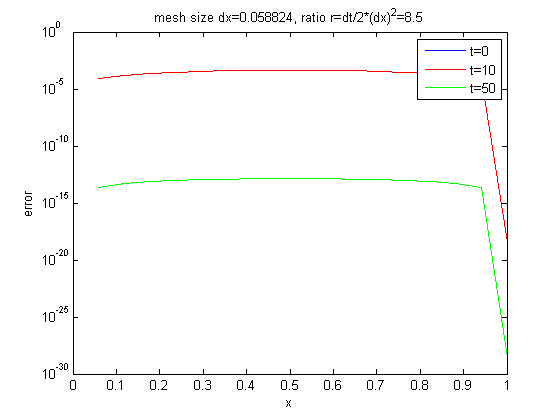
\includegraphics[width=.45\textwidth]{N_16logerror.png}}
\subfigure[{FD logerror for various time level when $N=32$ }]{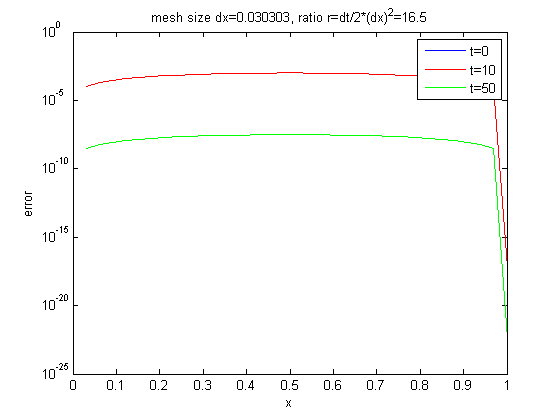
\includegraphics[width=.45\textwidth]{N_32logerror.png}}
\end{figure} 

%\begin{figure}
%\centering
%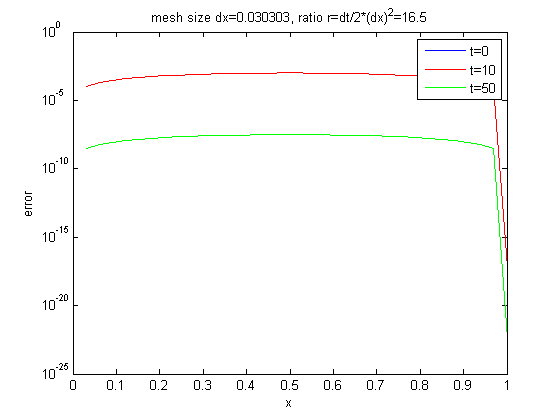
\includegraphics[width=.8\textwidth]{N_32logerror.png}
%\caption{FD logerror for various time level when $N=32$}
%\end{figure}

\begin{figure}
\centering
\subfigure[{FD solutions for various time level when $N=8$ and $dt=0.001$}]{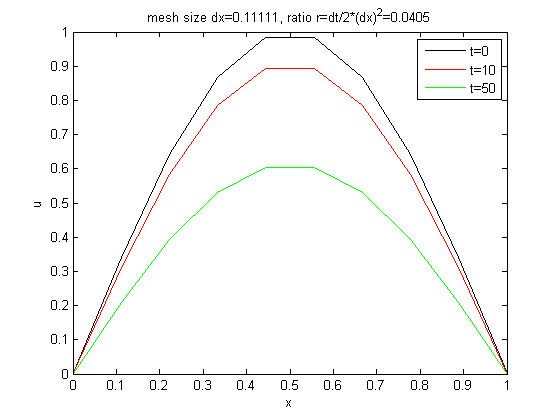
\includegraphics[width=.45\textwidth]{N_8fixdt.png}}
\subfigure[{FD solutions for various time level when $N=16$ and $dt=0.001$ }]{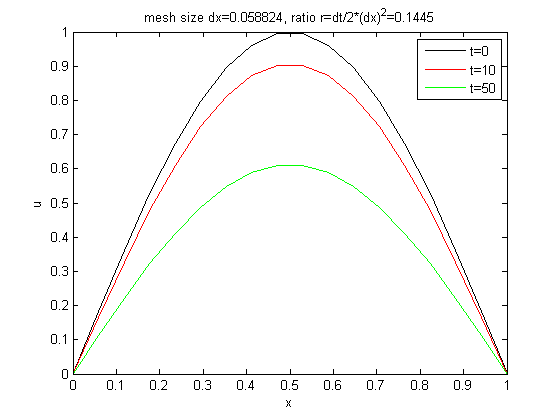
\includegraphics[width=.45\textwidth]{N_16fixdt.png}}
\end{figure} 


\begin{figure}
\centering
\subfigure[{FD solutions for various time level when $N=32$ and $dt=0.001$}]{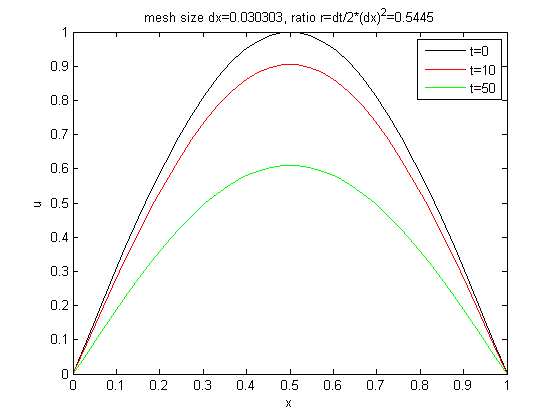
\includegraphics[width=.45\textwidth]{N_32fixdt.png}}
\subfigure[{FD surface plot when $N=8$ and $dt=0.001$}]{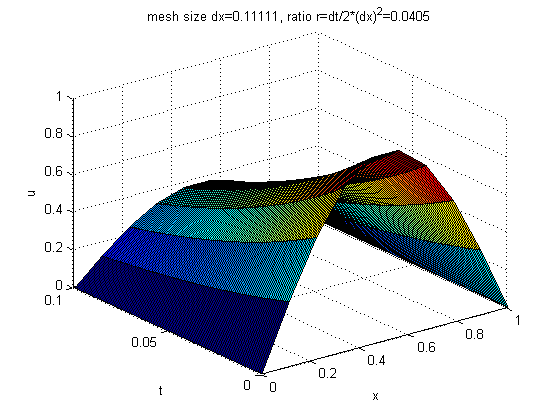
\includegraphics[width=.45\textwidth]{N_8surffixdt.png}}
\end{figure} 

\begin{figure}
\centering
\subfigure[{FD surface plot when $N=16$ and $dt=0.001$}]{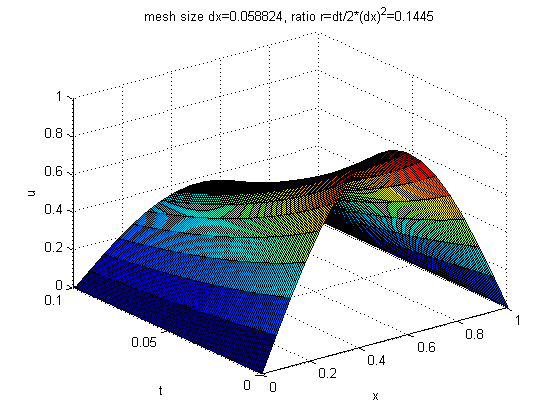
\includegraphics[width=.45\textwidth]{N_16surffixdt.png}}
\subfigure[{FD surface plot when $N=32$ and $dt=0.001$ }]{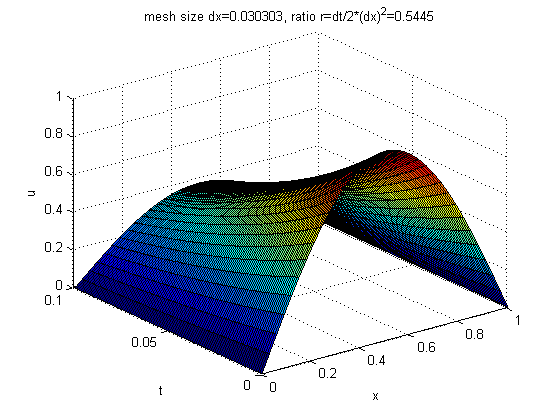
\includegraphics[width=.45\textwidth]{N_32surffixdt.png}}
\end{figure} 

\begin{figure}
\centering
\subfigure[{FD error for various time level when $N=8$ and $dt=0.001$}]{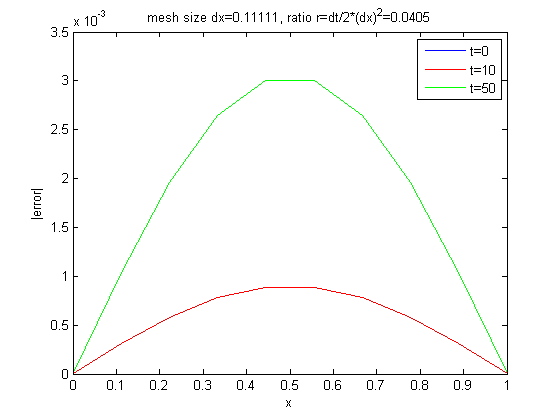
\includegraphics[width=.45\textwidth]{N_8errorfixdt.png}}
\subfigure[{FD error for various time level when $N=16$ and $dt=0.001$ }]{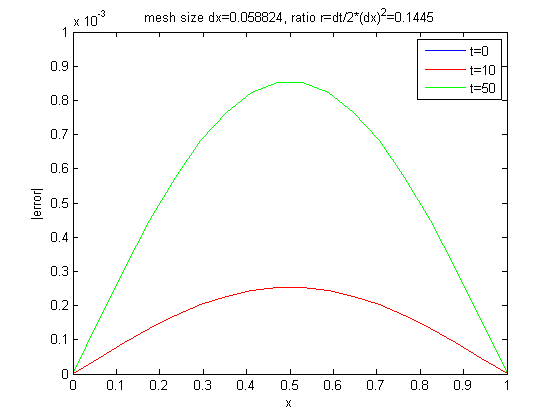
\includegraphics[width=.45\textwidth]{N_16errorfixdt.png}}
\end{figure} 

\begin{figure}
\centering
\subfigure[{FD error for various time level when $N=32$ and $dt=0.001$}]{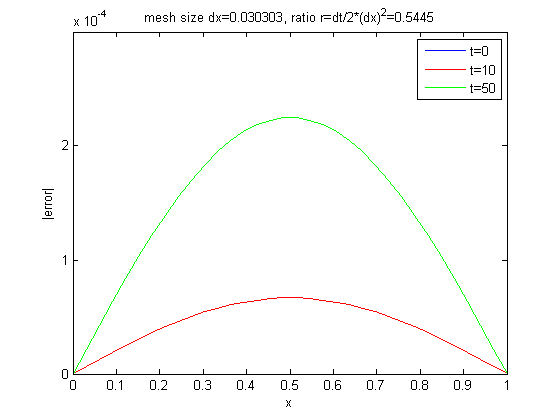
\includegraphics[width=.45\textwidth]{N_32errorfixdt.png}}
\subfigure[{FD logerror for various time level when $N=8$ and $dt=0.001$}]{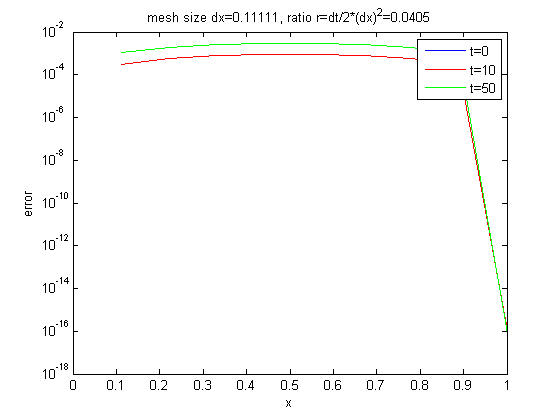
\includegraphics[width=.45\textwidth]{N_8logerrorfixdt.png}}
\end{figure}


\begin{figure}
\centering
\subfigure[{FD logerror for various time level when $N=16$ and $dt=0.001$}]{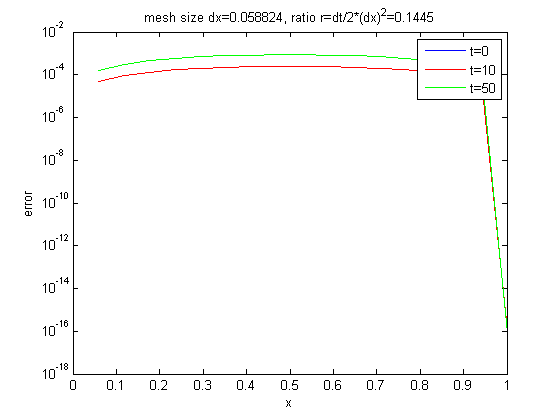
\includegraphics[width=.45\textwidth]{N_16logerrorfixdt.png}}
\subfigure[{FD logerror for various time level when $N=32$ and $dt=0.001$}]{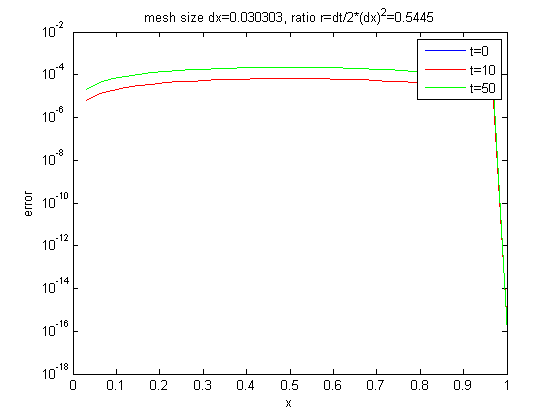
\includegraphics[width=.45\textwidth]{N_32logerrorfixdt.png}}
\end{figure} 


\end{enumerate}
\end{solution}